\documentclass[11pt]{article}

    \usepackage[breakable]{tcolorbox}
    \usepackage{parskip} % Stop auto-indenting (to mimic markdown behaviour)
    

    % Basic figure setup, for now with no caption control since it's done
    % automatically by Pandoc (which extracts ![](path) syntax from Markdown).
    \usepackage{graphicx}
    % Maintain compatibility with old templates. Remove in nbconvert 6.0
    \let\Oldincludegraphics\includegraphics
    % Ensure that by default, figures have no caption (until we provide a
    % proper Figure object with a Caption API and a way to capture that
    % in the conversion process - todo).
    \usepackage{caption}
    \DeclareCaptionFormat{nocaption}{}
    \captionsetup{format=nocaption,aboveskip=0pt,belowskip=0pt}

    \usepackage{float}
    \floatplacement{figure}{H} % forces figures to be placed at the correct location
    \usepackage{xcolor} % Allow colors to be defined
    \usepackage{enumerate} % Needed for markdown enumerations to work
    \usepackage{geometry} % Used to adjust the document margins
    \usepackage{amsmath} % Equations
    \usepackage{amssymb} % Equations
    \usepackage{textcomp} % defines textquotesingle
    % Hack from http://tex.stackexchange.com/a/47451/13684:
    \AtBeginDocument{%
        \def\PYZsq{\textquotesingle}% Upright quotes in Pygmentized code
    }
    \usepackage{upquote} % Upright quotes for verbatim code
    \usepackage{eurosym} % defines \euro

    \usepackage{iftex}
    \ifPDFTeX
        \usepackage[T1]{fontenc}
        \IfFileExists{alphabeta.sty}{
              \usepackage{alphabeta}
          }{
              \usepackage[mathletters]{ucs}
              \usepackage[utf8x]{inputenc}
          }
    \else
        \usepackage{fontspec}
        \usepackage{unicode-math}
    \fi

    \usepackage{fancyvrb} % verbatim replacement that allows latex
    \usepackage{grffile} % extends the file name processing of package graphics
                         % to support a larger range
    \makeatletter % fix for old versions of grffile with XeLaTeX
    \@ifpackagelater{grffile}{2019/11/01}
    {
      % Do nothing on new versions
    }
    {
      \def\Gread@@xetex#1{%
        \IfFileExists{"\Gin@base".bb}%
        {\Gread@eps{\Gin@base.bb}}%
        {\Gread@@xetex@aux#1}%
      }
    }
    \makeatother
    \usepackage[Export]{adjustbox} % Used to constrain images to a maximum size
    \adjustboxset{max size={0.9\linewidth}{0.9\paperheight}}

    % The hyperref package gives us a pdf with properly built
    % internal navigation ('pdf bookmarks' for the table of contents,
    % internal cross-reference links, web links for URLs, etc.)
    \usepackage{hyperref}
    % The default LaTeX title has an obnoxious amount of whitespace. By default,
    % titling removes some of it. It also provides customization options.
    \usepackage{titling}
    \usepackage{longtable} % longtable support required by pandoc >1.10
    \usepackage{booktabs}  % table support for pandoc > 1.12.2
    \usepackage{array}     % table support for pandoc >= 2.11.3
    \usepackage{calc}      % table minipage width calculation for pandoc >= 2.11.1
    \usepackage[inline]{enumitem} % IRkernel/repr support (it uses the enumerate* environment)
    \usepackage[normalem]{ulem} % ulem is needed to support strikethroughs (\sout)
                                % normalem makes italics be italics, not underlines
    \usepackage{soul}      % strikethrough (\st) support for pandoc >= 3.0.0
    \usepackage{mathrsfs}
    

    
    % Colors for the hyperref package
    \definecolor{urlcolor}{rgb}{0,.145,.698}
    \definecolor{linkcolor}{rgb}{.71,0.21,0.01}
    \definecolor{citecolor}{rgb}{.12,.54,.11}

    % ANSI colors
    \definecolor{ansi-black}{HTML}{3E424D}
    \definecolor{ansi-black-intense}{HTML}{282C36}
    \definecolor{ansi-red}{HTML}{E75C58}
    \definecolor{ansi-red-intense}{HTML}{B22B31}
    \definecolor{ansi-green}{HTML}{00A250}
    \definecolor{ansi-green-intense}{HTML}{007427}
    \definecolor{ansi-yellow}{HTML}{DDB62B}
    \definecolor{ansi-yellow-intense}{HTML}{B27D12}
    \definecolor{ansi-blue}{HTML}{208FFB}
    \definecolor{ansi-blue-intense}{HTML}{0065CA}
    \definecolor{ansi-magenta}{HTML}{D160C4}
    \definecolor{ansi-magenta-intense}{HTML}{A03196}
    \definecolor{ansi-cyan}{HTML}{60C6C8}
    \definecolor{ansi-cyan-intense}{HTML}{258F8F}
    \definecolor{ansi-white}{HTML}{C5C1B4}
    \definecolor{ansi-white-intense}{HTML}{A1A6B2}
    \definecolor{ansi-default-inverse-fg}{HTML}{FFFFFF}
    \definecolor{ansi-default-inverse-bg}{HTML}{000000}

    % common color for the border for error outputs.
    \definecolor{outerrorbackground}{HTML}{FFDFDF}

    % commands and environments needed by pandoc snippets
    % extracted from the output of `pandoc -s`
    \providecommand{\tightlist}{%
      \setlength{\itemsep}{0pt}\setlength{\parskip}{0pt}}
    \DefineVerbatimEnvironment{Highlighting}{Verbatim}{commandchars=\\\{\}}
    % Add ',fontsize=\small' for more characters per line
    \newenvironment{Shaded}{}{}
    \newcommand{\KeywordTok}[1]{\textcolor[rgb]{0.00,0.44,0.13}{\textbf{{#1}}}}
    \newcommand{\DataTypeTok}[1]{\textcolor[rgb]{0.56,0.13,0.00}{{#1}}}
    \newcommand{\DecValTok}[1]{\textcolor[rgb]{0.25,0.63,0.44}{{#1}}}
    \newcommand{\BaseNTok}[1]{\textcolor[rgb]{0.25,0.63,0.44}{{#1}}}
    \newcommand{\FloatTok}[1]{\textcolor[rgb]{0.25,0.63,0.44}{{#1}}}
    \newcommand{\CharTok}[1]{\textcolor[rgb]{0.25,0.44,0.63}{{#1}}}
    \newcommand{\StringTok}[1]{\textcolor[rgb]{0.25,0.44,0.63}{{#1}}}
    \newcommand{\CommentTok}[1]{\textcolor[rgb]{0.38,0.63,0.69}{\textit{{#1}}}}
    \newcommand{\OtherTok}[1]{\textcolor[rgb]{0.00,0.44,0.13}{{#1}}}
    \newcommand{\AlertTok}[1]{\textcolor[rgb]{1.00,0.00,0.00}{\textbf{{#1}}}}
    \newcommand{\FunctionTok}[1]{\textcolor[rgb]{0.02,0.16,0.49}{{#1}}}
    \newcommand{\RegionMarkerTok}[1]{{#1}}
    \newcommand{\ErrorTok}[1]{\textcolor[rgb]{1.00,0.00,0.00}{\textbf{{#1}}}}
    \newcommand{\NormalTok}[1]{{#1}}

    % Additional commands for more recent versions of Pandoc
    \newcommand{\ConstantTok}[1]{\textcolor[rgb]{0.53,0.00,0.00}{{#1}}}
    \newcommand{\SpecialCharTok}[1]{\textcolor[rgb]{0.25,0.44,0.63}{{#1}}}
    \newcommand{\VerbatimStringTok}[1]{\textcolor[rgb]{0.25,0.44,0.63}{{#1}}}
    \newcommand{\SpecialStringTok}[1]{\textcolor[rgb]{0.73,0.40,0.53}{{#1}}}
    \newcommand{\ImportTok}[1]{{#1}}
    \newcommand{\DocumentationTok}[1]{\textcolor[rgb]{0.73,0.13,0.13}{\textit{{#1}}}}
    \newcommand{\AnnotationTok}[1]{\textcolor[rgb]{0.38,0.63,0.69}{\textbf{\textit{{#1}}}}}
    \newcommand{\CommentVarTok}[1]{\textcolor[rgb]{0.38,0.63,0.69}{\textbf{\textit{{#1}}}}}
    \newcommand{\VariableTok}[1]{\textcolor[rgb]{0.10,0.09,0.49}{{#1}}}
    \newcommand{\ControlFlowTok}[1]{\textcolor[rgb]{0.00,0.44,0.13}{\textbf{{#1}}}}
    \newcommand{\OperatorTok}[1]{\textcolor[rgb]{0.40,0.40,0.40}{{#1}}}
    \newcommand{\BuiltInTok}[1]{{#1}}
    \newcommand{\ExtensionTok}[1]{{#1}}
    \newcommand{\PreprocessorTok}[1]{\textcolor[rgb]{0.74,0.48,0.00}{{#1}}}
    \newcommand{\AttributeTok}[1]{\textcolor[rgb]{0.49,0.56,0.16}{{#1}}}
    \newcommand{\InformationTok}[1]{\textcolor[rgb]{0.38,0.63,0.69}{\textbf{\textit{{#1}}}}}
    \newcommand{\WarningTok}[1]{\textcolor[rgb]{0.38,0.63,0.69}{\textbf{\textit{{#1}}}}}


    % Define a nice break command that doesn't care if a line doesn't already
    % exist.
    \def\br{\hspace*{\fill} \\* }
    % Math Jax compatibility definitions
    \def\gt{>}
    \def\lt{<}
    \let\Oldtex\TeX
    \let\Oldlatex\LaTeX
    \renewcommand{\TeX}{\textrm{\Oldtex}}
    \renewcommand{\LaTeX}{\textrm{\Oldlatex}}
    % Document parameters
    % Document title
    \title{R\_GSoC2026\_Proposal}
    
    
    
    
    
    
    
% Pygments definitions
\makeatletter
\def\PY@reset{\let\PY@it=\relax \let\PY@bf=\relax%
    \let\PY@ul=\relax \let\PY@tc=\relax%
    \let\PY@bc=\relax \let\PY@ff=\relax}
\def\PY@tok#1{\csname PY@tok@#1\endcsname}
\def\PY@toks#1+{\ifx\relax#1\empty\else%
    \PY@tok{#1}\expandafter\PY@toks\fi}
\def\PY@do#1{\PY@bc{\PY@tc{\PY@ul{%
    \PY@it{\PY@bf{\PY@ff{#1}}}}}}}
\def\PY#1#2{\PY@reset\PY@toks#1+\relax+\PY@do{#2}}

\@namedef{PY@tok@w}{\def\PY@tc##1{\textcolor[rgb]{0.73,0.73,0.73}{##1}}}
\@namedef{PY@tok@c}{\let\PY@it=\textit\def\PY@tc##1{\textcolor[rgb]{0.24,0.48,0.48}{##1}}}
\@namedef{PY@tok@cp}{\def\PY@tc##1{\textcolor[rgb]{0.61,0.40,0.00}{##1}}}
\@namedef{PY@tok@k}{\let\PY@bf=\textbf\def\PY@tc##1{\textcolor[rgb]{0.00,0.50,0.00}{##1}}}
\@namedef{PY@tok@kp}{\def\PY@tc##1{\textcolor[rgb]{0.00,0.50,0.00}{##1}}}
\@namedef{PY@tok@kt}{\def\PY@tc##1{\textcolor[rgb]{0.69,0.00,0.25}{##1}}}
\@namedef{PY@tok@o}{\def\PY@tc##1{\textcolor[rgb]{0.40,0.40,0.40}{##1}}}
\@namedef{PY@tok@ow}{\let\PY@bf=\textbf\def\PY@tc##1{\textcolor[rgb]{0.67,0.13,1.00}{##1}}}
\@namedef{PY@tok@nb}{\def\PY@tc##1{\textcolor[rgb]{0.00,0.50,0.00}{##1}}}
\@namedef{PY@tok@nf}{\def\PY@tc##1{\textcolor[rgb]{0.00,0.00,1.00}{##1}}}
\@namedef{PY@tok@nc}{\let\PY@bf=\textbf\def\PY@tc##1{\textcolor[rgb]{0.00,0.00,1.00}{##1}}}
\@namedef{PY@tok@nn}{\let\PY@bf=\textbf\def\PY@tc##1{\textcolor[rgb]{0.00,0.00,1.00}{##1}}}
\@namedef{PY@tok@ne}{\let\PY@bf=\textbf\def\PY@tc##1{\textcolor[rgb]{0.80,0.25,0.22}{##1}}}
\@namedef{PY@tok@nv}{\def\PY@tc##1{\textcolor[rgb]{0.10,0.09,0.49}{##1}}}
\@namedef{PY@tok@no}{\def\PY@tc##1{\textcolor[rgb]{0.53,0.00,0.00}{##1}}}
\@namedef{PY@tok@nl}{\def\PY@tc##1{\textcolor[rgb]{0.46,0.46,0.00}{##1}}}
\@namedef{PY@tok@ni}{\let\PY@bf=\textbf\def\PY@tc##1{\textcolor[rgb]{0.44,0.44,0.44}{##1}}}
\@namedef{PY@tok@na}{\def\PY@tc##1{\textcolor[rgb]{0.41,0.47,0.13}{##1}}}
\@namedef{PY@tok@nt}{\let\PY@bf=\textbf\def\PY@tc##1{\textcolor[rgb]{0.00,0.50,0.00}{##1}}}
\@namedef{PY@tok@nd}{\def\PY@tc##1{\textcolor[rgb]{0.67,0.13,1.00}{##1}}}
\@namedef{PY@tok@s}{\def\PY@tc##1{\textcolor[rgb]{0.73,0.13,0.13}{##1}}}
\@namedef{PY@tok@sd}{\let\PY@it=\textit\def\PY@tc##1{\textcolor[rgb]{0.73,0.13,0.13}{##1}}}
\@namedef{PY@tok@si}{\let\PY@bf=\textbf\def\PY@tc##1{\textcolor[rgb]{0.64,0.35,0.47}{##1}}}
\@namedef{PY@tok@se}{\let\PY@bf=\textbf\def\PY@tc##1{\textcolor[rgb]{0.67,0.36,0.12}{##1}}}
\@namedef{PY@tok@sr}{\def\PY@tc##1{\textcolor[rgb]{0.64,0.35,0.47}{##1}}}
\@namedef{PY@tok@ss}{\def\PY@tc##1{\textcolor[rgb]{0.10,0.09,0.49}{##1}}}
\@namedef{PY@tok@sx}{\def\PY@tc##1{\textcolor[rgb]{0.00,0.50,0.00}{##1}}}
\@namedef{PY@tok@m}{\def\PY@tc##1{\textcolor[rgb]{0.40,0.40,0.40}{##1}}}
\@namedef{PY@tok@gh}{\let\PY@bf=\textbf\def\PY@tc##1{\textcolor[rgb]{0.00,0.00,0.50}{##1}}}
\@namedef{PY@tok@gu}{\let\PY@bf=\textbf\def\PY@tc##1{\textcolor[rgb]{0.50,0.00,0.50}{##1}}}
\@namedef{PY@tok@gd}{\def\PY@tc##1{\textcolor[rgb]{0.63,0.00,0.00}{##1}}}
\@namedef{PY@tok@gi}{\def\PY@tc##1{\textcolor[rgb]{0.00,0.52,0.00}{##1}}}
\@namedef{PY@tok@gr}{\def\PY@tc##1{\textcolor[rgb]{0.89,0.00,0.00}{##1}}}
\@namedef{PY@tok@ge}{\let\PY@it=\textit}
\@namedef{PY@tok@gs}{\let\PY@bf=\textbf}
\@namedef{PY@tok@ges}{\let\PY@bf=\textbf\let\PY@it=\textit}
\@namedef{PY@tok@gp}{\let\PY@bf=\textbf\def\PY@tc##1{\textcolor[rgb]{0.00,0.00,0.50}{##1}}}
\@namedef{PY@tok@go}{\def\PY@tc##1{\textcolor[rgb]{0.44,0.44,0.44}{##1}}}
\@namedef{PY@tok@gt}{\def\PY@tc##1{\textcolor[rgb]{0.00,0.27,0.87}{##1}}}
\@namedef{PY@tok@err}{\def\PY@bc##1{{\setlength{\fboxsep}{\string -\fboxrule}\fcolorbox[rgb]{1.00,0.00,0.00}{1,1,1}{\strut ##1}}}}
\@namedef{PY@tok@kc}{\let\PY@bf=\textbf\def\PY@tc##1{\textcolor[rgb]{0.00,0.50,0.00}{##1}}}
\@namedef{PY@tok@kd}{\let\PY@bf=\textbf\def\PY@tc##1{\textcolor[rgb]{0.00,0.50,0.00}{##1}}}
\@namedef{PY@tok@kn}{\let\PY@bf=\textbf\def\PY@tc##1{\textcolor[rgb]{0.00,0.50,0.00}{##1}}}
\@namedef{PY@tok@kr}{\let\PY@bf=\textbf\def\PY@tc##1{\textcolor[rgb]{0.00,0.50,0.00}{##1}}}
\@namedef{PY@tok@bp}{\def\PY@tc##1{\textcolor[rgb]{0.00,0.50,0.00}{##1}}}
\@namedef{PY@tok@fm}{\def\PY@tc##1{\textcolor[rgb]{0.00,0.00,1.00}{##1}}}
\@namedef{PY@tok@vc}{\def\PY@tc##1{\textcolor[rgb]{0.10,0.09,0.49}{##1}}}
\@namedef{PY@tok@vg}{\def\PY@tc##1{\textcolor[rgb]{0.10,0.09,0.49}{##1}}}
\@namedef{PY@tok@vi}{\def\PY@tc##1{\textcolor[rgb]{0.10,0.09,0.49}{##1}}}
\@namedef{PY@tok@vm}{\def\PY@tc##1{\textcolor[rgb]{0.10,0.09,0.49}{##1}}}
\@namedef{PY@tok@sa}{\def\PY@tc##1{\textcolor[rgb]{0.73,0.13,0.13}{##1}}}
\@namedef{PY@tok@sb}{\def\PY@tc##1{\textcolor[rgb]{0.73,0.13,0.13}{##1}}}
\@namedef{PY@tok@sc}{\def\PY@tc##1{\textcolor[rgb]{0.73,0.13,0.13}{##1}}}
\@namedef{PY@tok@dl}{\def\PY@tc##1{\textcolor[rgb]{0.73,0.13,0.13}{##1}}}
\@namedef{PY@tok@s2}{\def\PY@tc##1{\textcolor[rgb]{0.73,0.13,0.13}{##1}}}
\@namedef{PY@tok@sh}{\def\PY@tc##1{\textcolor[rgb]{0.73,0.13,0.13}{##1}}}
\@namedef{PY@tok@s1}{\def\PY@tc##1{\textcolor[rgb]{0.73,0.13,0.13}{##1}}}
\@namedef{PY@tok@mb}{\def\PY@tc##1{\textcolor[rgb]{0.40,0.40,0.40}{##1}}}
\@namedef{PY@tok@mf}{\def\PY@tc##1{\textcolor[rgb]{0.40,0.40,0.40}{##1}}}
\@namedef{PY@tok@mh}{\def\PY@tc##1{\textcolor[rgb]{0.40,0.40,0.40}{##1}}}
\@namedef{PY@tok@mi}{\def\PY@tc##1{\textcolor[rgb]{0.40,0.40,0.40}{##1}}}
\@namedef{PY@tok@il}{\def\PY@tc##1{\textcolor[rgb]{0.40,0.40,0.40}{##1}}}
\@namedef{PY@tok@mo}{\def\PY@tc##1{\textcolor[rgb]{0.40,0.40,0.40}{##1}}}
\@namedef{PY@tok@ch}{\let\PY@it=\textit\def\PY@tc##1{\textcolor[rgb]{0.24,0.48,0.48}{##1}}}
\@namedef{PY@tok@cm}{\let\PY@it=\textit\def\PY@tc##1{\textcolor[rgb]{0.24,0.48,0.48}{##1}}}
\@namedef{PY@tok@cpf}{\let\PY@it=\textit\def\PY@tc##1{\textcolor[rgb]{0.24,0.48,0.48}{##1}}}
\@namedef{PY@tok@c1}{\let\PY@it=\textit\def\PY@tc##1{\textcolor[rgb]{0.24,0.48,0.48}{##1}}}
\@namedef{PY@tok@cs}{\let\PY@it=\textit\def\PY@tc##1{\textcolor[rgb]{0.24,0.48,0.48}{##1}}}

\def\PYZbs{\char`\\}
\def\PYZus{\char`\_}
\def\PYZob{\char`\{}
\def\PYZcb{\char`\}}
\def\PYZca{\char`\^}
\def\PYZam{\char`\&}
\def\PYZlt{\char`\<}
\def\PYZgt{\char`\>}
\def\PYZsh{\char`\#}
\def\PYZpc{\char`\%}
\def\PYZdl{\char`\$}
\def\PYZhy{\char`\-}
\def\PYZsq{\char`\'}
\def\PYZdq{\char`\"}
\def\PYZti{\char`\~}
% for compatibility with earlier versions
\def\PYZat{@}
\def\PYZlb{[}
\def\PYZrb{]}
\makeatother


    % For linebreaks inside Verbatim environment from package fancyvrb.
    \makeatletter
        \newbox\Wrappedcontinuationbox
        \newbox\Wrappedvisiblespacebox
        \newcommand*\Wrappedvisiblespace {\textcolor{red}{\textvisiblespace}}
        \newcommand*\Wrappedcontinuationsymbol {\textcolor{red}{\llap{\tiny$\m@th\hookrightarrow$}}}
        \newcommand*\Wrappedcontinuationindent {3ex }
        \newcommand*\Wrappedafterbreak {\kern\Wrappedcontinuationindent\copy\Wrappedcontinuationbox}
        % Take advantage of the already applied Pygments mark-up to insert
        % potential linebreaks for TeX processing.
        %        {, <, #, %, $, ' and ": go to next line.
        %        _, }, ^, &, >, - and ~: stay at end of broken line.
        % Use of \textquotesingle for straight quote.
        \newcommand*\Wrappedbreaksatspecials {%
            \def\PYGZus{\discretionary{\char`\_}{\Wrappedafterbreak}{\char`\_}}%
            \def\PYGZob{\discretionary{}{\Wrappedafterbreak\char`\{}{\char`\{}}%
            \def\PYGZcb{\discretionary{\char`\}}{\Wrappedafterbreak}{\char`\}}}%
            \def\PYGZca{\discretionary{\char`\^}{\Wrappedafterbreak}{\char`\^}}%
            \def\PYGZam{\discretionary{\char`\&}{\Wrappedafterbreak}{\char`\&}}%
            \def\PYGZlt{\discretionary{}{\Wrappedafterbreak\char`\<}{\char`\<}}%
            \def\PYGZgt{\discretionary{\char`\>}{\Wrappedafterbreak}{\char`\>}}%
            \def\PYGZsh{\discretionary{}{\Wrappedafterbreak\char`\#}{\char`\#}}%
            \def\PYGZpc{\discretionary{}{\Wrappedafterbreak\char`\%}{\char`\%}}%
            \def\PYGZdl{\discretionary{}{\Wrappedafterbreak\char`\$}{\char`\$}}%
            \def\PYGZhy{\discretionary{\char`\-}{\Wrappedafterbreak}{\char`\-}}%
            \def\PYGZsq{\discretionary{}{\Wrappedafterbreak\textquotesingle}{\textquotesingle}}%
            \def\PYGZdq{\discretionary{}{\Wrappedafterbreak\char`\"}{\char`\"}}%
            \def\PYGZti{\discretionary{\char`\~}{\Wrappedafterbreak}{\char`\~}}%
        }
        % Some characters . , ; ? ! / are not pygmentized.
        % This macro makes them "active" and they will insert potential linebreaks
        \newcommand*\Wrappedbreaksatpunct {%
            \lccode`\~`\.\lowercase{\def~}{\discretionary{\hbox{\char`\.}}{\Wrappedafterbreak}{\hbox{\char`\.}}}%
            \lccode`\~`\,\lowercase{\def~}{\discretionary{\hbox{\char`\,}}{\Wrappedafterbreak}{\hbox{\char`\,}}}%
            \lccode`\~`\;\lowercase{\def~}{\discretionary{\hbox{\char`\;}}{\Wrappedafterbreak}{\hbox{\char`\;}}}%
            \lccode`\~`\:\lowercase{\def~}{\discretionary{\hbox{\char`\:}}{\Wrappedafterbreak}{\hbox{\char`\:}}}%
            \lccode`\~`\?\lowercase{\def~}{\discretionary{\hbox{\char`\?}}{\Wrappedafterbreak}{\hbox{\char`\?}}}%
            \lccode`\~`\!\lowercase{\def~}{\discretionary{\hbox{\char`\!}}{\Wrappedafterbreak}{\hbox{\char`\!}}}%
            \lccode`\~`\/\lowercase{\def~}{\discretionary{\hbox{\char`\/}}{\Wrappedafterbreak}{\hbox{\char`\/}}}%
            \catcode`\.\active
            \catcode`\,\active
            \catcode`\;\active
            \catcode`\:\active
            \catcode`\?\active
            \catcode`\!\active
            \catcode`\/\active
            \lccode`\~`\~
        }
    \makeatother

    \let\OriginalVerbatim=\Verbatim
    \makeatletter
    \renewcommand{\Verbatim}[1][1]{%
        %\parskip\z@skip
        \sbox\Wrappedcontinuationbox {\Wrappedcontinuationsymbol}%
        \sbox\Wrappedvisiblespacebox {\FV@SetupFont\Wrappedvisiblespace}%
        \def\FancyVerbFormatLine ##1{\hsize\linewidth
            \vtop{\raggedright\hyphenpenalty\z@\exhyphenpenalty\z@
                \doublehyphendemerits\z@\finalhyphendemerits\z@
                \strut ##1\strut}%
        }%
        % If the linebreak is at a space, the latter will be displayed as visible
        % space at end of first line, and a continuation symbol starts next line.
        % Stretch/shrink are however usually zero for typewriter font.
        \def\FV@Space {%
            \nobreak\hskip\z@ plus\fontdimen3\font minus\fontdimen4\font
            \discretionary{\copy\Wrappedvisiblespacebox}{\Wrappedafterbreak}
            {\kern\fontdimen2\font}%
        }%

        % Allow breaks at special characters using \PYG... macros.
        \Wrappedbreaksatspecials
        % Breaks at punctuation characters . , ; ? ! and / need catcode=\active
        \OriginalVerbatim[#1,codes*=\Wrappedbreaksatpunct]%
    }
    \makeatother

    % Exact colors from NB
    \definecolor{incolor}{HTML}{303F9F}
    \definecolor{outcolor}{HTML}{D84315}
    \definecolor{cellborder}{HTML}{CFCFCF}
    \definecolor{cellbackground}{HTML}{F7F7F7}

    % prompt
    \makeatletter
    \newcommand{\boxspacing}{\kern\kvtcb@left@rule\kern\kvtcb@boxsep}
    \makeatother
    \newcommand{\prompt}[4]{
        {\ttfamily\llap{{\color{#2}[#3]:\hspace{3pt}#4}}\vspace{-\baselineskip}}
    }
    

    
    % Prevent overflowing lines due to hard-to-break entities
    \sloppy
    % Setup hyperref package
    \hypersetup{
      breaklinks=true,  % so long urls are correctly broken across lines
      colorlinks=true,
      urlcolor=urlcolor,
      linkcolor=linkcolor,
      citecolor=citecolor,
      }
    % Slightly bigger margins than the latex defaults
    
    \geometry{verbose,tmargin=1in,bmargin=1in,lmargin=1in,rmargin=1in}
    
    

\begin{document}
    
    \maketitle
    
    

    
    \hypertarget{project-info}{%
\subsection{Project Info}\label{project-info}}

\textbf{Project title:} hyperSpec-HPC: Fast Sparse Spectral Kernels in R
and Rust

\textbf{Project short title (30 characters):} Fast graph-based smoothing

\textbf{URL of project idea page:}
\url{github.com/rstats-gsoc/gsoc2026/wiki/hyperSpec‐HPC}

    \hypertarget{bio}{%
\subsection{Bio}\label{bio}}

I am Tamaghna Chattopadhyay, a pre-final year student pursuing a B.Tech
in Electronics Engineering at IIT(BHU) Varanasi. I have a deep interest
in Systems programming and Mathematics. I like to study and understand
the working and complexities of different algorithms. As a Electronics
student, I have learnt about spectroscopy and filtering through my
coursework. These subjects sparked my interest because of the rich
mathematical foundations behind them and their practical applications in
analyzing real-world signals. I have worked on various lab projects
involving filtering and image processing using Python. Additionally, I
am an upcoming Systems Intern at Nvidia and have worked as a embedded
systems engineer at a startup before.

I was first introduced to R through a university workshop where we were
taught the basics and given some tasks. Later, I explored R and its
packages on my own and used it on some personal work related to data
analysis. I have learnt Rust programming by myself through
\href{https://app.codecrafters.io/tracks/rust}{code crafters} and the
Rust Book (yet to fully finish), and worked on a Rust CLI from scratch
project.

I had contributed to some open source projects, most notable
contributions in Jenkins and Meshery, with around 20+ merged PRs.
Through these contributions, I had learned to work and be comfortable
with large codebases. Last year, I applied to Jenkins for GSoC with a
\href{https://drive.google.com/file/d/1NjQ4nWY_jHtc0QaP2AHDvc2LqZ3Bvswv/view?usp=sharing}{proposal}
focused on refactoring and optimizing the backend of an infrastructure
tool. Unfortunately, the project was not shortlisted due to a lack of
mentors, and I was not selected. However, the experience motivated me to
improve my skills and continue to work on myself.

    \hypertarget{contact-information}{%
\subsection{Contact Information}\label{contact-information}}

\textbf{Contributor name:} Tamaghna Chattopadhyay

\textbf{Contributor postal address:} 64 N.S. Avenue, Serampore, Hooghly,
West Bengal, India, 712201.

\textbf{Telephone(s):} +91-9674889722

\textbf{Email(s):} chattopadhyaytamaghna@gmail.com,
tamaghna.c.ece23@itbhu.ac.in

\textbf{Other communications channels:}\\
Hangouts: chattopadhyaytamaghna@gmail.com\\
Discord: tommichan101

    \hypertarget{contributor-affiliation}{%
\subsection{Contributor Affiliation}\label{contributor-affiliation}}

\textbf{Institution:} Indian Institute of Technology (BHU), Varanasi,
India

\textbf{Program:} B.Tech. in Electronics Engineering

\textbf{Stage of completion:} Third Year, expected completion in 2027

\textbf{Contact to verify:} Dr.~Amritanshu Pandey, head.ece@iitbhu.ac.in

    \hypertarget{schedule-conflicts}{%
\subsection{Schedule Conflicts}\label{schedule-conflicts}}

I do not have any major conflicts that will affect the project. I have a
summer break of more than 2 months and will be able to dedicate 40+
hours/week to R GSoC. The first week of May will be a bit tight as I
will be having my end semester exams, but I have planned ahead to
compensate for that. I have discussed the project goals with my mentor
and worked on certain parts of the project.

    \hypertarget{mentors}{%
\subsection{Mentors}\label{mentors}}

\textbf{Evaluating mentor name and email:} Erick Oduniyi
(eeoduniyi@gmail.com)

\textbf{Co-mentor name(s) and email(s):}

I have been in touch with Erick Oduniyi through Email, starting March,
2, 2026.

    \hypertarget{coding-plan-and-methods}{%
\section{Coding Plan and Methods}\label{coding-plan-and-methods}}

\hypertarget{project-background}{%
\subsection{Project Background}\label{project-background}}

The hyperSpec package provides a suite of tools for working with
spectroscopic data in R and is widely used for analyzing hyperspectral
datasets such as Raman and NIR imaging. While the package has evolved
significantly over the years, undergoing fortification in GSoC 2020, the
computational backend remains a bottleneck for large datasets. Many
operations such as spectral filtering, baseline correction, and
dimensionality reduction are currently implemented in pure R or rely on
dense matrix computations, which do not scale efficiently for large
hyperspectral images. Hyperspectral images naturally contain spatial
structure, where neighboring pixels often share similar chemical
properties. This makes them well suited for graph-based processing,
where pixels are treated as nodes and spatial adjacency defines edges.
Using the graph Laplacian, spatial smoothing can reduce noise while
preserving spectral feature.

Hyperspectral datasets can be extremely large (e.g., 512 x 512 pixels x
2048 wavelengths, roughly around 4 GB), and thus pure R implementations
begin to struggle. This project proposes implementing a Rust-powered
backend for sparse Laplacian spatial smoothing. By using efficient
sparse solvers with O(N) complexity, the Rust implementation can
significantly outperform the pure-R approaches.

\hypertarget{project-goal}{%
\subsection{Project Goal}\label{project-goal}}

The goal of this project is to implement a high-performance Rust backend
for graph-based spatial smoothing of hyperspectral images. This will
include creation of a new \texttt{hyperspec.rust} R package via extendr
with CI and basic tests, and implementing a reliable bridge between R's
\texttt{dgCMatrix} sparse matrix format and Rust's \texttt{faer} sparse
matrix representation. The Rust side will construct pixel neighborhood
graphs using \texttt{petgraph} and implement a sparse Laplacian solver
using \texttt{faer} iterative solvers (CG/BiCGSTAB) to compute the
smoothing operation \((I + αL)x = b\).

An R-level S4 method \textbf{graphSmooth(hy, alpha, neighbors)} will
expose the functionality to users. The Rust implementation will generate
adjacency graphs based on configurable neighborhood connectivity (e.g.,
4 or 8-connectivity) to minimize data transfer from R.

The project will also include performance benchmarks to compare the Rust
kernel with pure-R implementation for large hyperspectral datasets
(e.g., 512×512×2048, \textasciitilde4GB) and a vignette to demonstrate
spatial smoothing of hyperspectral Raman maps using graph filtering.

\textbf{Some extra goals that we plan to complete:}\\
i. Publishing the hyperSpec-HPC package to CRAN\\
ii. Publishing the dgCMatrix → faer FFI bridge pattern as Rust crate\\
iii. Publishing a JOSS paper documenting the package(s)

\textbf{The FFI challenge}\\
A key challenge in this project is handling the Foreign Function
Interface between R and Rust. R stores sparse matrices using the
\texttt{dgCMatrix} format, which uses a Compressed Sparse Column (CSC)
representation with three slots: i (row indices), p (column pointers),
and x (values). Since extendr does not provide a native zero-copy
wrapper for dgCMatrix, these components must be manually extracted from
R and safely wrapped as Rust slices to construct a corresponding sparse
matrix using the \texttt{faer} library. This requires careful validation
of the data and pointers, as incorrect handling can crash the R session.
There is a lot more on the FFI problem one could write about and it was
best understood after reading the IEEE paper draft shared by the mentor.

\hypertarget{workflow-diagram}{%
\subsubsection{Workflow Diagram}\label{workflow-diagram}}

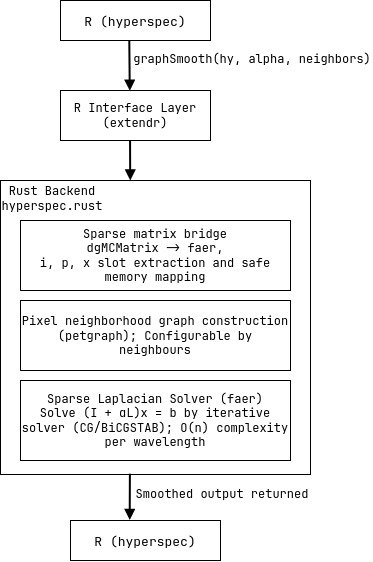
\includegraphics{diagrams/workflowR.jpg}

    \hypertarget{project-planning}{%
\subsection{Project Planning}\label{project-planning}}

The project will be planned and implemented in different stages. The
first stage is understanding the existing problem and the technical
challenges we might face. In traditional approaches (such as 1D
FFT-based filtering or Savitzky--Golay smoothing), they operate
independently on each pixel's spectrum. We plan to exploit the spatial
relationships present in hyperspectral data and reduce the time and
space complexities.

\textbf{Comparison Table for smoothing using different methods}

\begin{longtable}[]{@{}
  >{\raggedright\arraybackslash}p{(\columnwidth - 6\tabcolsep) * \real{0.3457}}
  >{\raggedright\arraybackslash}p{(\columnwidth - 6\tabcolsep) * \real{0.1975}}
  >{\raggedright\arraybackslash}p{(\columnwidth - 6\tabcolsep) * \real{0.2346}}
  >{\raggedright\arraybackslash}p{(\columnwidth - 6\tabcolsep) * \real{0.2222}}@{}}
\toprule\noalign{}
\begin{minipage}[b]{\linewidth}\raggedright
Method
\end{minipage} & \begin{minipage}[b]{\linewidth}\raggedright
Time Complexity
\end{minipage} & \begin{minipage}[b]{\linewidth}\raggedright
Memory Complexity
\end{minipage} & \begin{minipage}[b]{\linewidth}\raggedright
Estimated Runtime
\end{minipage} \\
\midrule\noalign{}
\endhead
\bottomrule\noalign{}
\endlastfoot
Dense R (\texttt{solve}) & O(N³) & O(N²) & Impractical \\
Sparse R (\texttt{Matrix::solve}) & O(N\^{}1.5) & O(N) &
\textasciitilde1 hour \\
Sparse Rust (CG, \texttt{faer}) & O(N √k) & O(N) & \textless{} 60 sec \\
\end{longtable}

This helps us understand why the Rust implementation is necessary.

I have already covered the key concepts required for this project,
including Graph Signal Processing basics, the R--Rust FFI bridge, and
the libraries extendr and faer (already used in tests). With this
preliminary preparation completed, I will now proceed with the setup and
detailed implementation plan for the project.

\textbf{The following development cycle will be followed}

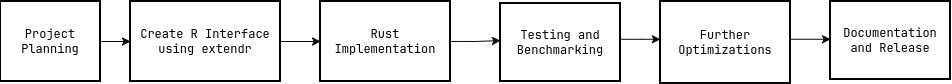
\includegraphics{diagrams/devcycle.jpg}

\hypertarget{setup}{%
\subsubsection{Setup}\label{setup}}

These are the libraries required for the project, on the R side, Rust
side, setup and testing tools. (Addional libraries may be needed as per
need).

\hypertarget{r-libraries}{%
\paragraph{R libraries}\label{r-libraries}}

\begin{enumerate}
\def\labelenumi{\arabic{enumi}.}
\tightlist
\item
  hyperSpec
\item
  extendr
\item
  usethis
\item
  devtools
\item
  Matrix
\item
  testthat
\end{enumerate}

\hypertarget{rust-libraries}{%
\paragraph{Rust libraries}\label{rust-libraries}}

\begin{enumerate}
\def\labelenumi{\arabic{enumi}.}
\tightlist
\item
  extendr\_api
\item
  faer
\item
  petgraph
\item
  thiserror
\end{enumerate}

    \hypertarget{implementation-plan}{%
\subsection{Implementation Plan}\label{implementation-plan}}

\hypertarget{stage-1-creation-of-hyperspec.rust-skeleton-with-ci-and-basic-tests}{%
\subsubsection{\texorpdfstring{Stage 1: Creation of
\texttt{hyperSpec.rust} skeleton with CI and basic
tests}{Stage 1: Creation of hyperSpec.rust skeleton with CI and basic tests}}\label{stage-1-creation-of-hyperspec.rust-skeleton-with-ci-and-basic-tests}}

This stage involves setting up a github repository/ contributing to the
existing codebase. I will maintain regular communication with my mentor
to ensure that the initial structure of the module aligns with the
project goals and existing architecture of the hyperSpec ecosystem. I
will discuss the proposed repository layout, the Rust--R integration
approach using extendr, and the setup of continuous integration (CI) for
automated builds and tests. Feedback from the mentor will help refine
the project skeleton, testing strategy, and coding conventions. We can
create the basic skeleton for the project using:

\begin{verbatim}
library(usethis)
library(rextendr)
usethis::create_package("hyperspec.rust")
setwd("hyperspec.rust")
rextendr::use_extendr()
\end{verbatim}

The generated project structure :

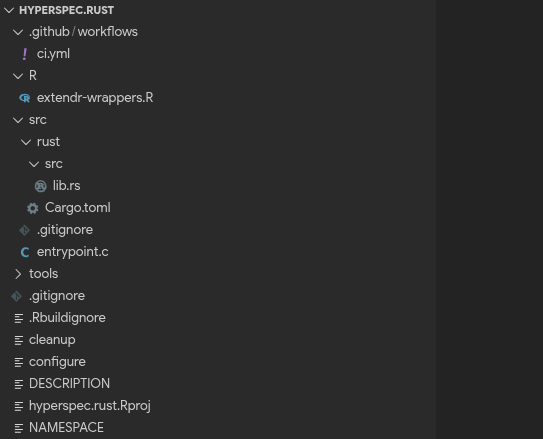
\includegraphics{diagrams/projstruc.png}

We add all our dependencies inside the
\texttt{hyperspec.rust/src/rust/Cargo.toml} file. Example:

\begin{verbatim}
[dependencies]
extendr-api = '0.7'
faer = "0.19"
\end{verbatim}

Along with that we can also setup some of the CI workflow using github
actions using a yaml file in \texttt{.github/workflows/} directory.

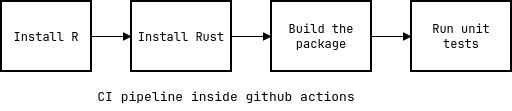
\includegraphics{diagrams/ci.jpg}

\hypertarget{stage-2-the-dgcmatrix-faer-sparse-matrix-bridge}{%
\subsubsection{Stage 2: The dgCMatrix → faer sparse matrix
bridge}\label{stage-2-the-dgcmatrix-faer-sparse-matrix-bridge}}

The extendr package, an R-to-Rust FFI library, does not provide a native
wrapper for \texttt{dgCMatrix}. This is the FFI problem and the we need
to tackle this by constructing a reliable bridge between R's
\texttt{dgCMatrix} sparse matrix representation and the sparse matrix
structures used by the Rust \texttt{faer} library. This bridge enables
high-performance graph-based computations on hyperspectral datasets
while maintaining compatibility with the existing hyperSpec ecosystem.\\
In R, sparse matrices from the \texttt{Matrix} package are stored using
the Compressed Sparse Column (CSC) representation through the dgCMatrix
S4 class. The CSC structure consists of three arrays: the \textbf{value
array x}, the \textbf{row index array i}, and the \textbf{column pointer
array p}. These arrays encode all non-zero elements of the matrix and
allow efficient traversal of columns. By extracting these arrays and
passing them through the extendr interface, the sparse matrix structure
can be reconstructed inside Rust using the faer sparse matrix API.

For better understanding the CSC representation, here is a example:

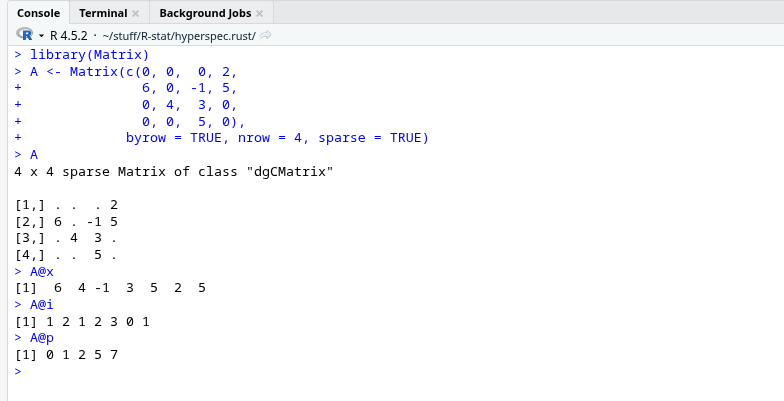
\includegraphics{diagrams/csceg.png}

\hypertarget{r-rust-ffi-bridge-implementation}{%
\paragraph{R-Rust FFI Bridge
Implementation}\label{r-rust-ffi-bridge-implementation}}

\hfill\break
\textbf{R side: Slot extraction}\\
Since extendr has no native \texttt{dgCMatrix} wrapper, we extract the
slots: x, i and p in R before calling the Rust function. This is not
zero copy as R allocates the slots before passing them. However, each
slot is a standard R vector and the transfer time is almost negligible
for sparse matrix.

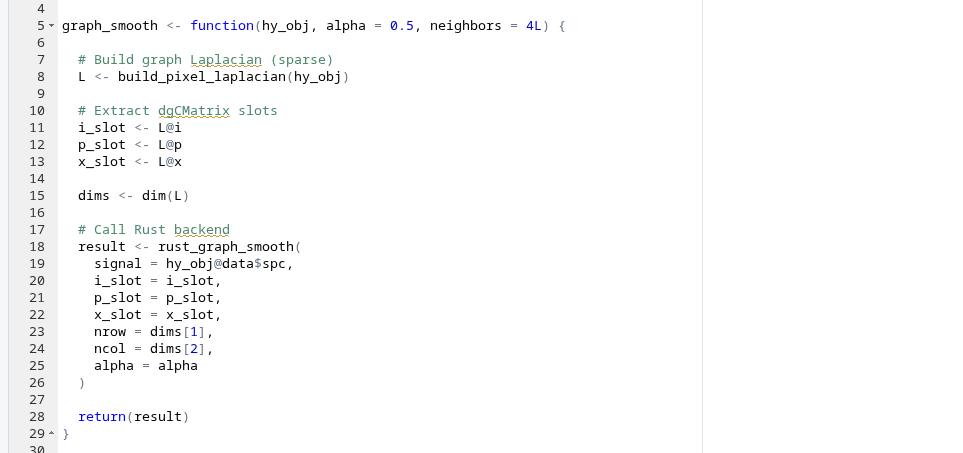
\includegraphics{diagrams/Rsideofbridge.png}

\textbf{Rust side: Reconstruction and Validation}\\
The Rust function reconstructs the sparse matrix and performs validation
before computation. Defensive checks before any pointer arithmetic
ensure that malformed input from R cannot cause memory errors.

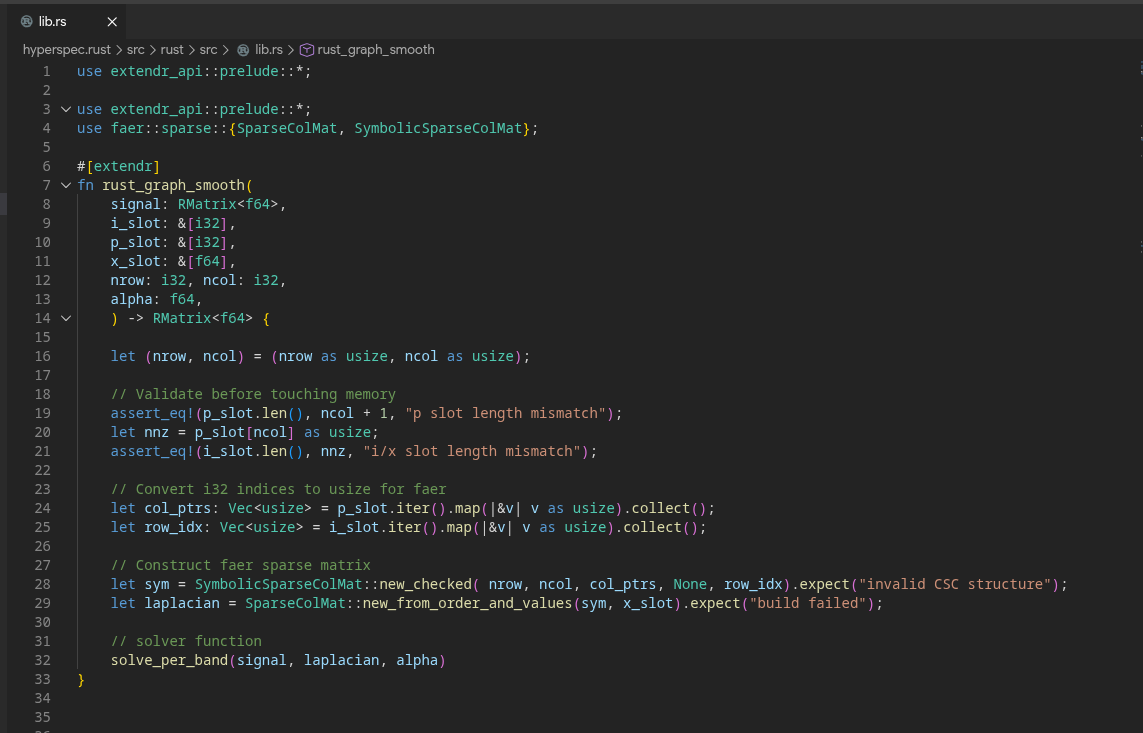
\includegraphics{diagrams/Rustside.png}

\textbf{Note:} R stores slots i and p as \texttt{int32}, whereas faer
expects \texttt{usize} in Rust. This conversion is safe (as
\(nnz < 2^{31}\) for any realistic sparse matrix), but needs be
explicit. Rust's ownership system prevents the most common Rcpp
failures:\\
\textbf{Buffer overflow:} Rust's slice indexing panics on out-of-bounds
access rather than reading adjacent memory.\\
\textbf{Use-after-free:} The borrow checker ensures R vectors passed to
Rust remain valid for the duration of the function call.

\hypertarget{stage-3-pixel-neighborhood-graph-construction}{%
\subsubsection{Stage 3: Pixel Neighborhood Graph
Construction}\label{stage-3-pixel-neighborhood-graph-construction}}

In hyperspectral spatial smoothing, the image is modeled as a graph
where each pixel is a node and edges connect neighboring pixels. This
graph captures the spatial structure of the image and forms the basis
for constructing the graph Laplacian matrix, which is later used in the
smoothing equation: \texttt{(I+αL)x=b}. The Rust library
\texttt{petgraph} is used to build this graph.

As seen earlier, the pixel neighborhood graph should be configurable by
the number of neighbors (e.g, 4 or 8) because different spatial models
require different connectivity. This is also consistent with the
material where the function accepts a parameter \texttt{neighbors} to
choose the connectivity.

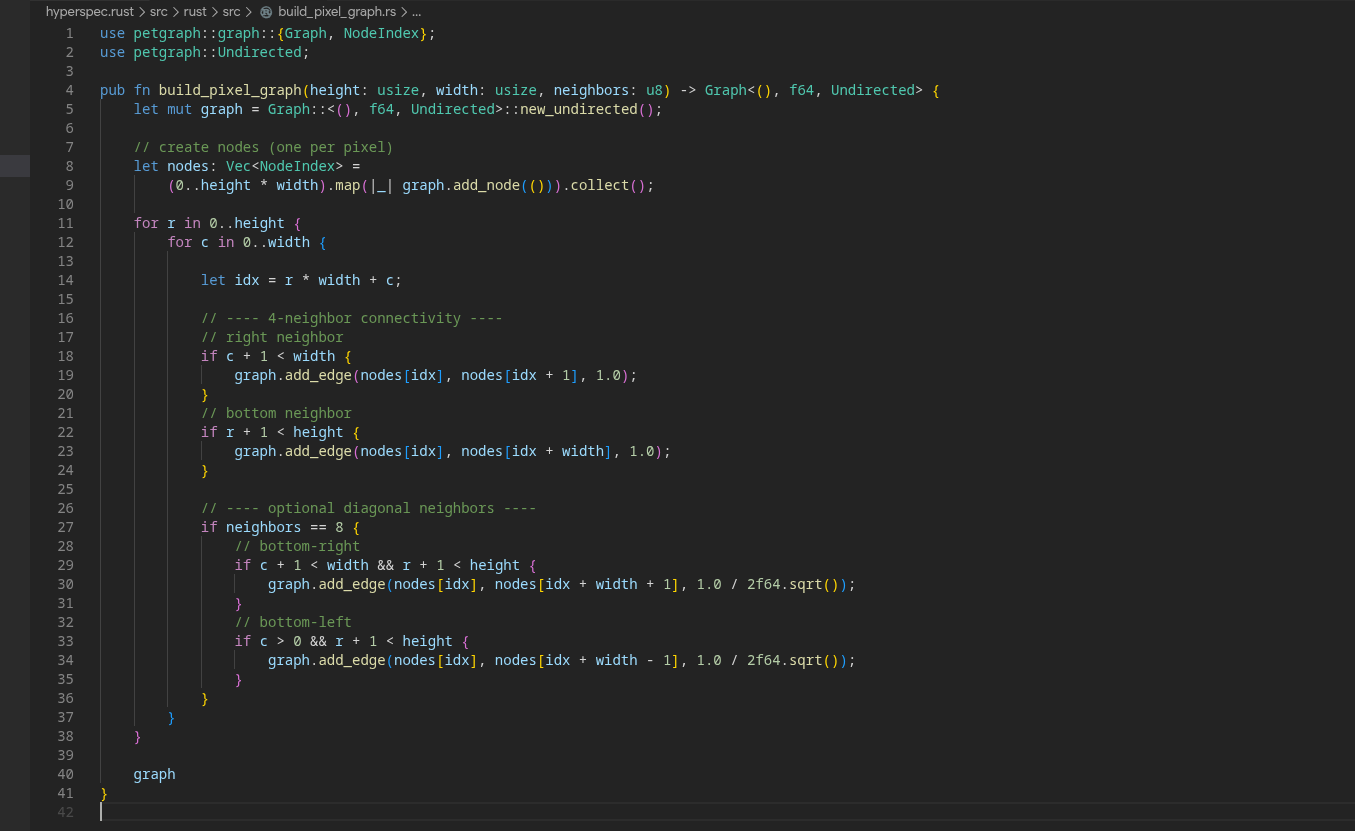
\includegraphics{diagrams/pixelneigh.png}

The types of connectivity we get from this:

\begin{longtable}[]{@{}lll@{}}
\toprule\noalign{}
neighbors & Connectivity & Description \\
\midrule\noalign{}
\endhead
\bottomrule\noalign{}
\endlastfoot
\texttt{4} & 4-neighborhood & horizontal + vertical pixels \\
\texttt{8} & 8-neighborhood & horizontal + vertical + diagonal \\
\end{longtable}

\textbf{Why connectivity matters?}\\
More neighbours means stronger spatial coupling, and hence smoother
results. 4 neighbors mean sharper edges preserved, while 8 neighbors
mean smoother results. The configuration may depend based on the type of
operation.

Once we have this, the Graph Laplacian can be computed using:
\(L = D − W\) where W = adjacency matrix and D = degree matrix.\\
This Laplacian is the core operator used in the smoothing system.
Instead of sending a huge adjacency matrix across the R--Rust FFI
boundary, Rust reconstructs the graph using only height, width,
connectivity. This greatly reduces FFI overhead.

You can check out this interactive figure to visualize the Laplacian
construction: link(TODO)

\hypertarget{stage-4-iterative-solver-using-cgbicgstab}{%
\subsubsection{Stage 4: Iterative Solver using
CG/BiCGSTAB}\label{stage-4-iterative-solver-using-cgbicgstab}}

Once the Laplacian is built, we need to perform graph-based low-pass
filtering, for reducing spatial noise while preserving large structures.
Spatial smoothing is formulated as solving the linear system
\[(I + αL)x = b\] for each wavelength band, where L is the graph
Laplacian, b is the original signal, x is the smoothed output, and
\(α > 0\) controls the smoothing strength.

Since L is sparse, the system can be solved efficiently using iterative
methods such as Conjugate Gradient (CG) for symmetric systems or
BiCGSTAB for non-symmetric systems. This reduces the computational
complexity to \textbf{\(O(N)\)} per band, compared to
\textbf{\(O(N^3)\)} for dense solvers. Both these methods are present in
the \texttt{faer} library.

\hypertarget{conjugate-gradient-algorithm}{%
\paragraph{Conjugate Gradient
Algorithm}\label{conjugate-gradient-algorithm}}

\hfill\break
If the matrix \(I + αL\) is symmetric, then we use this approach. The CG
method solves \(A_x = b\), where \(A = I + αL\). Then the algorithm
iteratively improves the solution.

Algorithm steps :-\\
i. Initialize \(x_0 = 0\)\\
ii. compute residual: \(r_0 = b - A x_0\)\\
iii. Update search direction: \(p_0 = r_0\)\\
iv. Iterate until convergence

\textbf{Rust implementation}

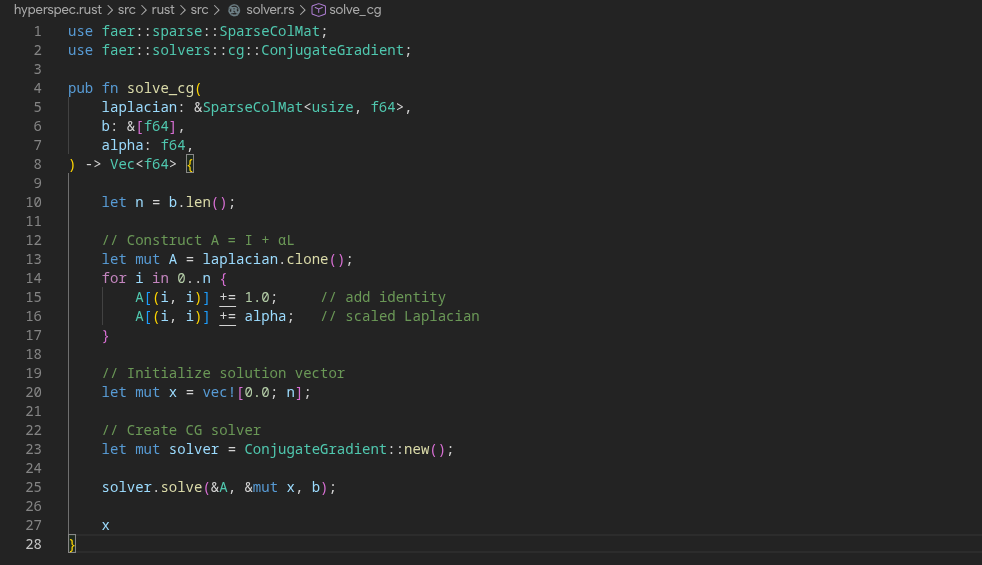
\includegraphics{diagrams/cg.png}

\hypertarget{bicgstab-bi-conjugate-gradient-stabilized-algorithm}{%
\paragraph{BiCGSTAB (Bi-Conjugate Gradient Stabilized)
Algorithm}\label{bicgstab-bi-conjugate-gradient-stabilized-algorithm}}

\hfill\break
If the matrix \(I + αL\) is non-symmetric, then we use this approach.

Algorithm :-\\
i. Initialize \(x_0 = 0\), \(r_0 = b - A x_0\)\\
ii. Choose a shadow residual \(\hat{r} = r_0\)\\
iii. Iteration: Compute intermediate scalars and vectors to update the
solution:\\
\hspace*{0.333em} update step size\\
\hspace*{0.333em} compute intermediate residual\\
\hspace*{0.333em} compute stabilization factor\\
iv. Update solution\\
v. Update residual and direction\\
vi. Update \(r_{k+1}\) and search direction, then repeat until
convergence.\\

\textbf{Rust implementation}

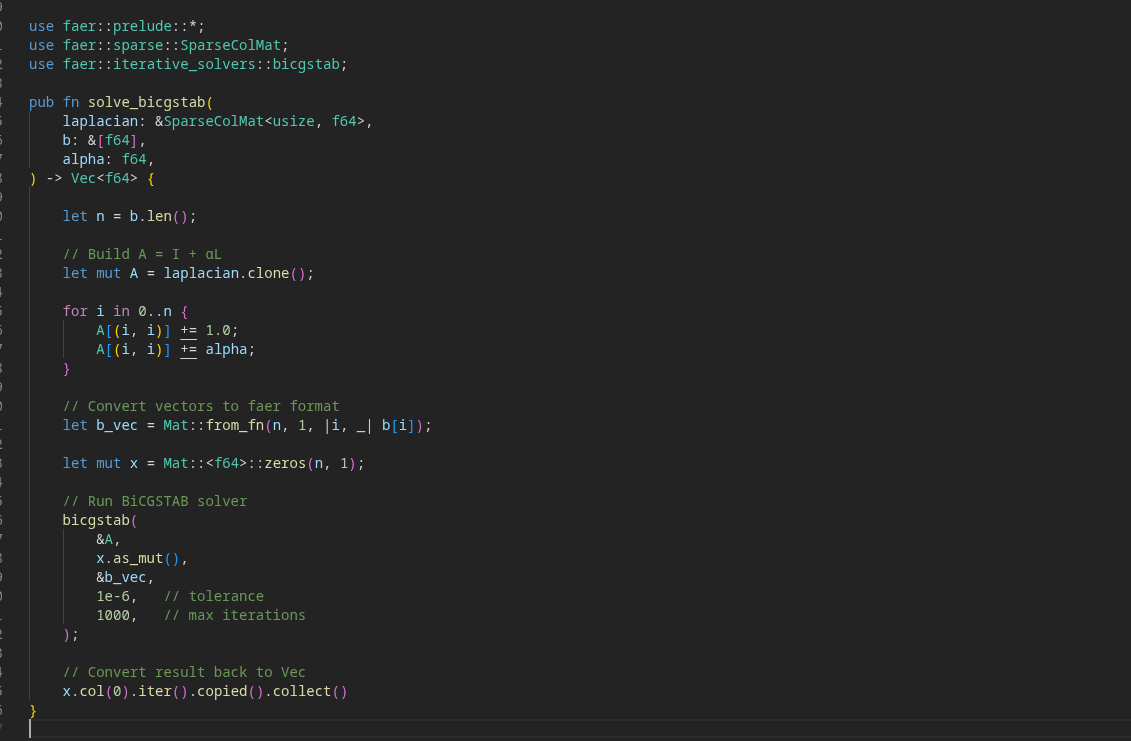
\includegraphics{diagrams/bigcstab.png}

\hypertarget{stage-5-parallel-spectral-processing}{%
\subsubsection{Stage 5: Parallel Spectral
Processing}\label{stage-5-parallel-spectral-processing}}

Hyperspectral images have many wavelength bands and each solver only
solves for one wavelength band. Each band requires solving a separate
system: \((I + \alpha L)x_k = b_k\)\\
These solves are completely independent, which means we can run them in
parallel using the \texttt{Rayon} library in Rust.

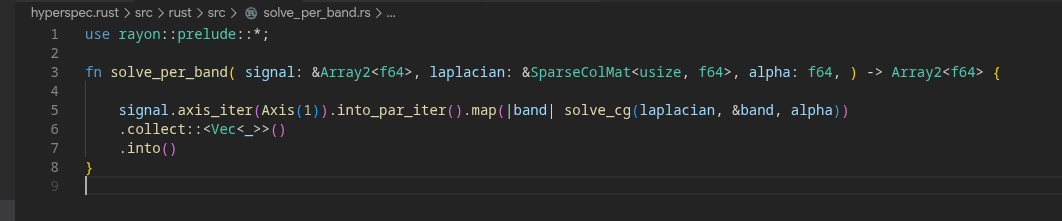
\includegraphics{diagrams/parallel.png}

\hypertarget{stage-6-testing-and-benchmarking}{%
\subsubsection{Stage 6: Testing and
Benchmarking}\label{stage-6-testing-and-benchmarking}}

\hypertarget{unit-tests}{%
\paragraph{Unit Tests}\label{unit-tests}}

\hfill\break
The testing strategy will combine unit tests, integration tests, and
performance benchmarks for large datasets. We use the \texttt{testthat}
package inside the module and add the testfiles in the
\texttt{hyperspec.rust/tests/testthat/} directory. Then we can run the
unit tests automatically using \texttt{devtools::test()}. The following
4 unit tests will validate each component of the Rust backend
independently:

\begin{enumerate}
\def\labelenumi{\arabic{enumi}.}
\tightlist
\item
  \textbf{FFI Bridge Validation:} The first component to test is the
  conversion from the R dgCMatrix sparse matrix format to Rust sparse
  structures. The following will be implemented:
\end{enumerate}

\begin{enumerate}
\def\labelenumi{\roman{enumi}.}
\tightlist
\item
  Correctness in extraction of i, p, and x slots from a dgCMatrix.
\item
  Verify: \texttt{length(i)\ ==\ length(x)},
  \texttt{length(p)\ ==\ ncol\ +\ 1}, column pointers are monotonic, row
  indices fall within valid bounds.
\item
  Proper descriptive error messages returned to R incase of any failure.
\end{enumerate}

\begin{enumerate}
\def\labelenumi{\arabic{enumi}.}
\setcounter{enumi}{1}
\tightlist
\item
  \textbf{Adjacency Graph Construction Tests:} The pixel adjacency graph
  will be tested to ensure correct connectivity. The following will be
  implemented:
\end{enumerate}

\begin{enumerate}
\def\labelenumi{\roman{enumi}.}
\tightlist
\item
  Correct number of nodes for a given grid size.
\item
  Correct number of edges depending on the type of connectivity (eg,
  4-connectivity or 8-connectivity).
\item
  Validate that interior, edge, and corner pixels have correct neighbor
  counts (eg, a corner pixel has 2 neighbors, edge pixel has 3).
\end{enumerate}

\begin{enumerate}
\def\labelenumi{\arabic{enumi}.}
\setcounter{enumi}{2}
\tightlist
\item
  \textbf{Laplacian Matrix Construction:} The Laplacian construction
  logic will be validated using small matrices. We first construct the
  Laplacian and then verify it's properties :
\end{enumerate}

\begin{enumerate}
\def\labelenumi{\roman{enumi}.}
\tightlist
\item
  diagonal elements equal the node degree.
\item
  off-diagonal entries equal −1 for neighbors
\item
  row sums equal zero for the Laplacian
\end{enumerate}

\begin{enumerate}
\def\labelenumi{\arabic{enumi}.}
\setcounter{enumi}{3}
\tightlist
\item
  \textbf{Corectness of the iterative solver:} The solver results will
  be validated for already known results calculated using dense R
  solver. There might be very small errors and hence we require a
  tolerence value(almost negligible) for the check.
\end{enumerate}

\hypertarget{integration-test}{%
\paragraph{Integration Test}\label{integration-test}}

\hfill\break
The Integration tests would verify that the entire processing pipeline:
from the R interface to the Rust solver and back to R. These tests will
be automated using Continuous Integration (CI) so they run on every
commit and pull request. The goal is to ensure:\\
i. The R interface with graphSmooth(hy, alpha, neighbors) works
correctly.\\
ii. FFI conversion does not crash the R session.\\
iii. Solver results are correct.\\
iv. Package builds successfully.

\textbf{Workflow Structure (inside \texttt{.github/workflows/ci.yml} )}

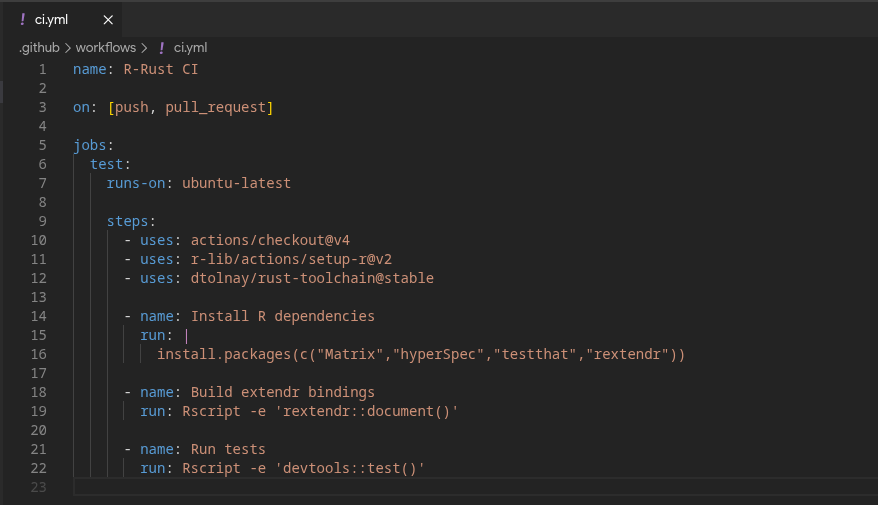
\includegraphics{diagrams/citest.png}

\hypertarget{benchmarks}{%
\paragraph{Benchmarks}\label{benchmarks}}

\hfill\break
The target benchmark is for a \textbf{512 × 512 × 2048} hyperspectral
dataset (approximately 4 GB). The 512 × 512 represents the spatial pixel
grid and 2048 represents the wavelength dimension. The pure-R
implementation has a time complexity of \(O(N^3)\) and a space
complexity of \(O(N^2)\). It would take up \textbf{hours to run and
about 16GB} of RAM on a laptop (honestly speaking my laptop might just
crash). The Rust implementation time complexity is O(N √k) and space
complexity is \(O(N)\), so it would be completed in \textbf{less than 1
minute with about 4GB RAM}.

\textbf{Baseline Comparison:} The Rust implementation will be compared
against a baseline pure-R approach using sparse matrix operations from
the \texttt{Matrix} package. In the baseline method, spatial smoothing
is performed by solving the linear system \((I+αL)x = b\) using standard
R numerical routines such as \texttt{Matrix::solve()}.

\hypertarget{documentaion}{%
\subsubsection{Documentaion}\label{documentaion}}

I will make a developer-friendly documentation for all the Rust
functions and the R level method including parameter explainations,
examples, performance notes, etc. The \texttt{roxygen} and
\texttt{knitr} packages will be used.

A detailed vignette will demonstrate the complete spatial smoothing
workflow on a hyperspectral Raman dataset, explaining the motivation for
graph-based filtering and the underlying Laplacian formulation
\((I+αL)x = b\). The \texttt{rmarkdown} package will be used and the
vignette will also include explanations of the Laplacian filtering
method, example code, and visualizations of results before and after
smoothing.

    \hypertarget{project-obstacles}{%
\subsection{Project Obstacles}\label{project-obstacles}}

No project plan is completely free from challenges, and I anticipate a
few possible obstacles during the development. One challenge may be
ensuring correct and efficient communication between R and Rust through
the extendr FFI interface, particularly when handling large
hyperspectral datasets. There might be misunderstandings while
understanding certain concepts or errors in implementing code.
Additionally, some components may take more time than initially
expected. To address these challenges, I plan to set small milestones,
maintain regular communication with the mentor and provide progress
reports for feedback. I will keep myself enthusiastic and complete the
work in time for a successful R GSoC experience.

    \hypertarget{timeline}{%
\section{Timeline}\label{timeline}}

\hypertarget{rough-timelime}{%
\subsection{Rough timelime}\label{rough-timelime}}

\begin{longtable}[]{@{}ll@{}}
\toprule\noalign{}
Date & Event \\
\midrule\noalign{}
\endhead
\bottomrule\noalign{}
\endlastfoot
March 31 - April 30 & Pre-GSoC Period \\
May 1 -- May 24 & Community Bonding Period \\
May 25 -- July 5 & Coding Period 1 \\
July 6 -- July 10 & Midterm Evaluations \\
July 11 -- August 16 & Coding Period 2 \\
August 17 - August 24 & Final Week \\
August 24 - August 31 & Endterm Evaluations \\
August 24 - November 2 & Incase of extended coding period \\
November 2 & Final Evaluations (extended) \\
November 11 & Program officially ends \\
\end{longtable}

I will try my best to complete the entire project within the standard
time period (before August 31), and have prepared the detailed timeline
accordingly.

\hypertarget{detailed-timeline}{%
\subsection{Detailed Timeline}\label{detailed-timeline}}

\hypertarget{pre-gsoc-period-march-31---april-30}{%
\subsubsection{Pre-GSoC Period (March 31 - April
30)}\label{pre-gsoc-period-march-31---april-30}}

\hypertarget{week-1}{%
\paragraph{Week 1}\label{week-1}}

\hfill\break
Study the \texttt{hyperSpec} repository and read all the R documentation
related to it. I will study graph signal processing and deepen my
understanding of the existing challenges in order to explore potential
optimization approaches. Setup all the neccessary development tools and
get familiar with using the different packages.

\hypertarget{week-2}{%
\paragraph{Week 2}\label{week-2}}

\hfill\break
Continue to spend time understanding the codebase and start solving open
issues in R. Read documentaation and study the implementations used in
various spectroscopic libraries and review the recent developments.

\hypertarget{week-3}{%
\paragraph{Week 3}\label{week-3}}

\hfill\break
Work on improving Rust proficiency. Read the documentation for faer
0.19+ sparse module, focusing on areas of the iterative solver APIs (CG
and BiCGSTAB). Read all documentation related to extendr and understand
how R S4 objects are handled at the FFI boundary. Read documentation of
petgraph and write some Rust code for graph construction and solver
experimentation.

\hypertarget{week-4}{%
\paragraph{Week 4}\label{week-4}}

\hfill\break
Strengthen my understanding of R fundamentals. Continue solving issues
and contributing. Read documentation and get familiar with the testing
libraries.

\hypertarget{community-bonding-period-may-1---may-24}{%
\subsubsection{Community Bonding Period (May 1 - May
24)}\label{community-bonding-period-may-1---may-24}}

\hypertarget{week-1-1}{%
\paragraph{Week 1}\label{week-1-1}}

\hfill\break
Establish a clear communication schedule with the mentor, including
weekly meetings, progress updates, and discussion channels for technical
questions. Finalize the project plan and set milestones for the project.
Discuss the development flow for setting up repository, forking,
branching, committing, and submitting pull requests.

\hypertarget{week-2-1}{%
\paragraph{Week 2}\label{week-2-1}}

\hfill\break
Understand the existing development practices used by the hyperSpec
project. Finalize the development environment and tools. Create the
initial \texttt{hyperspec.rust} skeleton, configure Continuous
Integration (CI), and implement a small Rust function callable from R to
verify that the Rust--R bridge works correctly. Download all datasets
required for testing and benchmarking.

\hypertarget{week-3-1}{%
\paragraph{Week 3}\label{week-3-1}}

\hfill\break
Complete stage 1 of the plan: Creation of hyperSpec.rust skeleton with
CI and basic tests. Continue reading the resources provided by my
mentor. Review the documentation and work on building a prototype for
the dgCMatrix → faer sparse matrix bridge.

\hypertarget{week-4-1}{%
\paragraph{Week 4}\label{week-4-1}}

\hfill\break
Continue reading the resources provided by my mentor. Finalize
everything with the mentor and share the report on the prototype.

\hypertarget{coding-period-1-may-25---july-5}{%
\subsubsection{Coding Period 1 (May 25 - July
5)}\label{coding-period-1-may-25---july-5}}

\hypertarget{week-1-2}{%
\paragraph{Week 1}\label{week-1-2}}

\hfill\break
Complete Stage 1 before the Coding Period. Start working on Stage 2: The
R-Rust FFI Bridge. Implement the R side and Rust side code for the
bridge. Share the weekly progress report with the mentor.

\hypertarget{week-2-2}{%
\paragraph{Week 2}\label{week-2-2}}

\hfill\break
Continue working on Stage 2. Add validation checks and error handling.
Verify correctness of the bridge and that the transfer is as intended.
Share the weekly progress report with the mentor.

\hypertarget{week-3-2}{%
\paragraph{Week 3}\label{week-3-2}}

\hfill\break
Start working on Stage 3: Pixel Neighborhood Graph Construction.
Implement the Rust code and verify correctness. Share the weekly
progress report with the mentor.

\hypertarget{week-4-2}{%
\paragraph{Week 4}\label{week-4-2}}

\hfill\break
Continue working on Stage 3. Implement flexible graph construction
configurable by neighbors. Optimize graph construction and validate
correctness for larger grids. Share the weekly progress report with the
mentor.

\hypertarget{week-5}{%
\paragraph{Week 5}\label{week-5}}

\hfill\break
Start working on Stage 4: Iterative Solver using CG/BiCGSTAB. Implement
solver (for symmetric case) in Rust using CG and verify correctness.
Share the weekly progress report with the mentor.

\hypertarget{week-6}{%
\paragraph{Week 6}\label{week-6}}

\hfill\break
Implement solver (for non-symmetric case) using BiCGSTAB. Wrap up
everything and complete Stage 4. Integrate the solver with the R
interface: \texttt{graphSmooth(hy,\ alpha,\ neighbors)} function
callable from R. Share the weekly progress report with the mentor.

\hypertarget{midterm-evaluations-july-6-july-10}{%
\subsubsection{Midterm Evaluations (July 6 -- July
10)}\label{midterm-evaluations-july-6-july-10}}

Write a detailed report on all the work done during the Coding Period.
All work will be documented and uploaded.\\
\textbf{Midterm Deliverables:}\\
i. hyperspec.rust package skeleton with CI and basic tests.\\
ii. dgCMatrix → faer sparse matrix bridge.\\
iii. Pixel adjacency graph construction.\\
iv. Sparse Laplacian solver in Rust.\\
v. Functional graphSmooth(hy, alpha, neighbors) R S4 method.

\hypertarget{coding-period-2-july-11-august-16}{%
\subsubsection{Coding Period 2 (July 11 -- August
16)}\label{coding-period-2-july-11-august-16}}

\hypertarget{week-1-3}{%
\paragraph{Week 1}\label{week-1-3}}

\hfill\break
The coding continues. Test the Spatial smoothing working on different
datasets and verify that output maintains proper structure. Start
working on Stage 5: Parallel Spectral Processing using rayon. Share the
weekly progress report with the mentor.

\hypertarget{week-2-3}{%
\paragraph{Week 2}\label{week-2-3}}

\hfill\break
Complete work on Stage 5. Test the solver for multiple wavebands
parallelly using different datasets. Share the weekly progress report
with the mentor.

\hypertarget{week-3-3}{%
\paragraph{Week 3}\label{week-3-3}}

\hfill\break
Start working on Stage 6: Testing and Benchmarking. Write unit tests for
the different components. Write Integration tests and put everything
together in the CI pipeline. Share the weekly progress report with the
mentor.

\hypertarget{week-4-3}{%
\paragraph{Week 4}\label{week-4-3}}

\hfill\break
Complete stage 6. Work on performance benchmarks using the 512 × 512 ×
2048 hyperspectral dataset. Compare pure-R and Rust sparse solver
results. Document all benchmark results and performance plots. Share the
weekly progress report with the mentor.

\hypertarget{week-5-1}{%
\paragraph{Week 5}\label{week-5-1}}

\hfill\break
Work on the last stage. Write detailed documentation and vignette to
demonstrate Spatial smoothing of hyperspectral Raman maps using graph
filtering. Share the weekly progress report with the mentor.

\hypertarget{final-week-august-17---august-24}{%
\subsubsection{Final Week (August 17 - August
24)}\label{final-week-august-17---august-24}}

Wrap up everything. Complete all documentation and any remaining work.
Optimize the functions further and refactor code. Test that everything
works successfully. Share the weekly progress report with the mentor.

\hypertarget{endterm-august-24---august-31}{%
\subsubsection{Endterm (August 24 - August
31)}\label{endterm-august-24---august-31}}

Write a complete project report on all the work done. Write about
performance improvements and tests. All work will be uploaded.\\
\textbf{Endterm Deliverables:}\\
i. Parallel Spectral Processing.\\
ii. Unit and Integration tests.\\
iii.Benchmarks and performance report.\\
iv. Complete documentation and vignette.

\hypertarget{contingency-plan}{%
\subsection{Contingency Plan}\label{contingency-plan}}

If any setbacks occur due to my health, personal or family reasons, I
will communicate with my mentor, explain the difficulty, and seek their
guidance on how to adjust the timeline. If technical issues or delays
occur during development, I will focus on completing the core components
first, particularly the dgCMatrix → faer sparse matrix bridge and the
basic sparse Laplacian solver, and then extend the implementation
gradually. There may be times, such as during exams, when I might not be
able to devote my full-time to the project. However, I will compensate
for that by working extra hard later on. I have kept around 2 weeks time
for managing each stage. If things go south, the schedule can be
adjusted by utilizing the extended period.

    \hypertarget{management-of-coding-project}{%
\section{Management of Coding
Project}\label{management-of-coding-project}}

I will track my progress through weekly reports. Additionally, I plan to
maintain a blog where I will regularly document updates, which will help
ensure that I stay aligned with the planned timeline. During the
Community Bonding Period, I will discuss and establish a meeting
schedule with my mentor and provide regular progress updates. I will
review and incorporate all feedback that is provided. I will commit code
several times a week, making sure that all changes are thoroughly tested
before each commit.

    \hypertarget{test}{%
\section{Test}\label{test}}

To get prepared for the project, I had done all the three tests(easy,
medium and hard) given by the mentor. Through the tests, I learned a lot
of things that would be useful for the project like computing pixel
adjacency matrix and using it to find the laplacian, creating R package
using extendr, writing tests using testthat in R, slot extraction from a
R dgCMatrix sparse matrix via extendr and constructing a faer sparse
matrix from it. All these tasks gave me experience in using the packages
and an insight into the mathematical concepts behind them. The tests
were really well designed and it was fun to do them. I made a small
writeup for the tasks, on how I solved them along with setup
instructions.

\hypertarget{easy-task}{%
\subsection{Easy Task}\label{easy-task}}

\textbf{Problem Statement:} Install hyperSpec in R. Load the flu or
laser dataset. Write a script that constructs a simple pixel adjacency
matrix from a 2D spatial grid and computes its graph Laplacian using
base R. Plot the result.\\
\textbf{Solution:}
https://github.com/shinigami-777/hyperSpec-Tasks/tree/main/easy\_task

\hypertarget{medium-task}{%
\subsection{Medium Task}\label{medium-task}}

\textbf{Problem Statement:} Create a minimal R package using extendr.
Pass a dense matrix from R to Rust, compute its row sums in Rust using
faer, and return the result to R. Include a test.\\
\textbf{Solution:}
https://github.com/shinigami-777/hyperSpec-Tasks/tree/main/medium\_task

\hypertarget{hard-task}{%
\subsection{Hard Task}\label{hard-task}}

\textbf{Problem Statement:} Extract the i, p, and x slots from an R
dgCMatrix sparse matrix via extendr. Wrap them as Rust slices and
construct a faer sparse matrix. Return the degree vector (row sums) to R
using extendr's WritableSlice to avoid an unnecessary allocation, and
verify it matches the pure-R result.\\
\textbf{Solution:}
https://github.com/shinigami-777/hyperSpec-Tasks/tree/main/hard\_task

\hypertarget{anything-else}{%
\section{Anything Else}\label{anything-else}}

\hypertarget{recent-work-related-to-project}{%
\subsection{Recent Work Related to
Project}\label{recent-work-related-to-project}}

I had worked on creating a Rust crate with reusable dgCMatrix → faer FFI
bridge pattern. Check out
\url{https://github.com/shinigami-777/dgcmatrix-faer-bridge}. This will
be very useful for the implementation of the FFI Bridge in the project
as we can directly use the crate/code.

\hypertarget{references}{%
\subsection{References}\label{references}}

{[}1{]} IEEE paper draft on dgCMatrix → faer FFI bridge by Erick
Oduniyi\\
{[}2{]} https://letters-photon-processor.web.app/sparse-bridge\\
{[}3{]} https://github.com/eoduniyi/sparse-bridge-visualizations\\
{[}4{]} https://github.com/rstats-gsoc/gsoc2026/wiki/hyperSpec-HPC\\
{[}5{]} https://eoduniyi.github.io/hyperSpec.gsoc2020/


    % Add a bibliography block to the postdoc
    
    
    
\end{document}
